\documentclass[
  msc,proposal,
  oneside,
  hidecover,
  hidededication,
  hideack,
  hideepigraph,
  hidelof,
  hidelot,
  hideabstract,
  hidecover,
  extraporttitlepagefalse
]{ppgccufmg}    

\usepackage[english]{babel}
\usepackage[latin1]{inputenc}
\usepackage[T1]{fontenc}
\usepackage{type1ec}
\usepackage{graphicx}
\usepackage[a4paper,
  portuguese,
  bookmarks=true,
  bookmarksnumbered=true,
  linktocpage,
  colorlinks,
  citecolor=black,
  urlcolor=black,
  linkcolor=black,
  filecolor=black,
  ]{hyperref}
\usepackage[square]{natbib}

\begin{document}

\ppgccufmg{
  title={Web data extraction in semi-structured documents},
  authorrev={de Freitas Veneroso, Jo�o Mateus},
  cutter={D1234p},
  cdu={519.6*82.10},
  university={Federal University of Minas Gerais},
  course={Computer Science},
  address={Belo Horizonte},
  date={2017-11},
  advisor={Berthier Ribeiro de Ara�jo Neto},
  approval={img/approvalsheet.eps}
}

% ==========================================
% Beginning of text.                       |
% ==========================================

\chapter{Introduction}

Web data extraction is the task of automatically extracting structured information
from unstructured or semi-structured web documents. It is a subset of the broader
field of Information Extraction, and thus it faces many of the same challenges. 

Structured information such as that found in a well organized relational database must 
conform to an underlying data model, namely an abstract model that formalizes
the entities and relationships in a given application domain. Unstructured information
however is not organized according to a logical model, therefore useful bits of data won't
be arranged cohesively and will ocasionally be permeated by chunks of irrelevant information.

Tipically, Information Extraction tasks consist of mapping unstructured or poorly
structured data to a semantically well defined structure. The input is usually
composed of a set of documents that describe a group of entities in a similar manner,
while the Information Extraction task deals with identifying those entities and 
organizing them according to a template. 

As an example, consider a collection of 
novels and the task of identifying the name of the main character in each novel. 
For this task, the model must first identify proper nouns and then understand the 
text sufficiently to allow inference on the relative importance of each noun. 

To achieve such a goal it is often useful to employ methods developed in the disciplines 
of Information Retrieval and Natural Language Processing. The former has achieved a 
great deal of success in the task of classifying documents according to statistical 
properties and the latter led to huge improvements in modelling human language.
Many times, the various methods employed in these disciplines lead to different 
approaches in the field of Information Extraction.

In the scope of this work, we are interested in the semi-structured data usually
found in HTML web documents. Web documents most often lie in between the 
structured-unstructured data paradigm, meaning that they take a rather
relaxed approach in regard to formal structure. Hierarchy, element disposition,
class names, and other features related to document structure and indirectly associated
with the data itself are valuable information in the task of identifying entities and 
determining relationships. So much that many times they are the major source of information 
for classification purposes, such as when extracting information from standardized tables.
However, far from a structured database, web documents usually provide very limited structure
to otherwise unstructured data such as that found in free text.

Our current focused research interest regarding web data extraction is collecting
computer science researcher information from university websites. We need this 
information in order to compare the reputations of national and international 
research groups in the area of computer science with the academic reputation ranking
metric proposed by \cite{Ribas2015} based on random walks over reputation graphs. 

It showed promising results when ranking publication venues and 
individual authors in the area of Computer Science by using information publically available in 
the DBLP repository (http://dblp.uni-trier.de/). However the DBLP database has sparse information 
about author affiliation and multiple records are outdated. To remedy this problem, in the past 
few years researchers from UFMG have been laboriously collecting this data manually, however
this process is tedious and inefficient. Currently, we only have affiliation information for 
about 1\% of the authors, being most of them from USA and Brazil and this is not nearly enough to 
allow broad international research group comparison.

Up to now, our goal has been to build an automatic information extraction system for
collecting author affiliation information from university websites. It has already 
achieved significant progress which shall be described further in section 3. However, the ideas 
developed in this concrete case will be further improved in order to construct a more general
approach to the broader Information Extraction task.

The research here described hopes to contribute by proposing a novel approach to the main 
Information Extraction task, making the computer science affiliation database available for 
further research and testing the quality of academic reputation metrics regarding 
research groups.

\chapter{Related Work}

In the last 20 years, the exponential growth of public information in the web has 
led to the development of a number of different approaches to the problem of web 
data extraction. Traditionally, the task was solved by designing special purpose
programs called wrappers to pinpoint relevant data and store it in some structured
format. The multiple tools varied wildly according to their degree of automation. 

It was readily perceived that manual wrapper generation was a rather tedious and
error prone process, unsuited for large scale operations. Already in 2000,
\cite{Kushmerick2000} advocated for wrapper induction, a technique for automatically
constructing wrappers. This approach is known in the literature by the acronym 
WIEN (Wrapper Induction ENvironment).

Web data extraction techniques often require some sort of assistance from human 
experts to boost accuracy. So the main challenge in the field lies in determining
an adequate tradeoff between degree of automation and precision.

In 2002, a survey by \cite{Laender2002} made a thorough classification of the
early approaches with a taxonomy based on their main technology, being them: languages for
wrapper development, HTML-aware tools, NLP-based tools, Wrapper Induction Tools,
Modeling-based tools and Ontology-based tools. Some noteworthy examples from this era
are: 

TSIMMIS \cite{Hammer1997} and WebOQL \cite{Arocena1999}, which are special purpose 
languages for building wrappers.

Road Runner \cite{Crescenzi2001}, XWRAP \cite{Liu2000} and W4F \cite{Sahuguet1999}, 
which are HTML-aware tools that infer meaningful patterns from the HTML structure.

RAPIER \cite{Califf1999}, SRV \cite{Freitag1998}, WHISK \cite{Soderland1999}, which 
are NLP-based tools.

WIEN \cite{Kushmeric2000}, Soft Mealy \cite{Hsu1998} and STALKER \cite{Muslea1999} which 
are wrapper induction methods.

NoDoSE \cite{Adelberg1998} and Debye \cite{Laender2002a}, which are semi supervised modeling
based tools that require some interaction with the user by means of a graphical
user interface.

In 2004, \cite{Flesca2004} developed a taxonomy emphasizing the advantages and 
drawbacks of web data extraction technologies according to the user viewpoint.
In 2006 \cite{Chang2006} complemented the previous surveys with new technologies.

In 2008 \cite{Sarawagi2008} classifies wrappers in the following three types: 
record-level, page-level and site-level wrappers. Record-level wrappers are only
able to process single records, page-level wrappers are capable of 
extracting data from a single page, and site-level wrappers are able to process
the whole webpage structure including subpages and their linking structure.

More recently, surveys by \cite{Ferrara2014} and \cite{Schulz2016} updated the 
previous surveys and included new approaches.

In 2016 \cite{Varlamov2016}, argued that the degree of automation can no
longer be the main classification criterion for the data extraction systems
because unsupervised methods which were widely considered to be the state 
of the art when dealing with individual websites performed poorly or were
innapropriate on cross site extraction tasks. The authors proposed a 
classification of methods by the extent of their application. 
The competing approaches were separated into two groups: methods for individual 
websites and methods that are applicable to whole application domains. 

The first group contains most of the earlier approaches, including the supervised
approaches: SRV \cite{Freitag1998}, RAPIER \cite{Califf1999}, WHISK \cite{Soderland1999}, 
WIEN \cite{Kushmeric2000} SoftMealy \cite{Hsu1998} and STALKER \cite{Muslea1999}; and
the unsupervised approaches: RoadRunner \cite{Crescenzi2001} and EXALG \cite{Arasu2003}.

The second group is divided between domain specific methods and domain agnostic methods.
Domain specific methods are designed for extracting data about a particular 
application domain across multiple websites. Our researcher name extractor 
method that will be further described in section 3 falls in this category. Domain
specific methods integrate information about the particular application domain in the 
course of its development and thus are able to achieve superior performance in
comparison to domain agnostic methods.

Domain agnostic methods are the most general extraction methods. They can extract
information from any application domain from multiple websites. They pose the hardest
challenge because the tool must infer data relevance without any prior training in
thar particular application domain. Some examples are: ODE \cite{Su2009}, ObjectRunner 
\cite{Abdessalem2010}, and AMBER \cite{Furche2012}.

Our method is finely tuned for the researcher name extraction task, however it is 
our intent to create a more general agnostic method based 
on statistical properties in future research.

\chapter{Methodology}

This section describes briefly a statistical NLP approach to solve the researcher 
affiliation extraction problem presented in section 1. This problem is actually
composed of two parts. The first one envolves crawling university websites and
finding faculty repositories and the second one is extracting the actual researcher
affiliation data from these repositories. 

The crawling

The crawling problem has been partially solved by online aggregators that
compiled university internet domains for most of the academic world. One of these
aggregators is https://univ.cc/, which contains links for the main websites of
9553 universities from 207 countries. These root domains were fed as seeds to
our crawler, that downloaded the entire websites and its subdomains, amounting
around 2 million documents. Once all webpages were downloaded the task at hand 
becomes identifying faculty repositories among the downloaded pages. 

This task can be accomplished quite efficiently by means of supervised machine
learning models once we have labeled a subset of the university webpages.
The labeling was manually done for 2440 pages, of which 373 were faculty repositories
and 2067 were other types of pages. We took care to select a proportional number
of pages from each country.

Since the classification task is not our main research focus, the results will
only be presented here briefly. Our classifier employed 112 features:
60 were the number of occurrences of a set of relevant keywords in the URL, the page 
title, h1, h2 and h3 tags. Each element having its own set of features.
49 where the number of occurrences of a different set of keywords in the rest of the
text of the page.
1 feature measured the document length
1 feature was the number of names found by a simplified version of our name extractor.

\begin{tabular}{ l c r }
  Random Forest & 0.93 & 0.02 \\
  Gaussian Naive Bayes & 0.88 & 0.03 \\
  SVM & 0.85 & 0.05 \\
  Logistic Regression & 0.90 & 0.02 \\
\end{tabular}

Four models were tested by means of 5 fold cross validation, the results are presented in
table 1. All models except Support Vector Machines achieved a reasonable performance,
however, since the Random Forest Classifier presented a more stable predictive capability,
it was chosen as the classifier method for labeling the remaining webpages.

Data extraction

The data extraction stage consists of extracting researcher names from faculty directories.
The main challenge here is constructing a general enough approach that can be used 
effectively across different domains without extracting too much garbage together with the
valuable information. This task faces a typical precision vs. recall tradeoff.

\begin{figure}
  \centering
  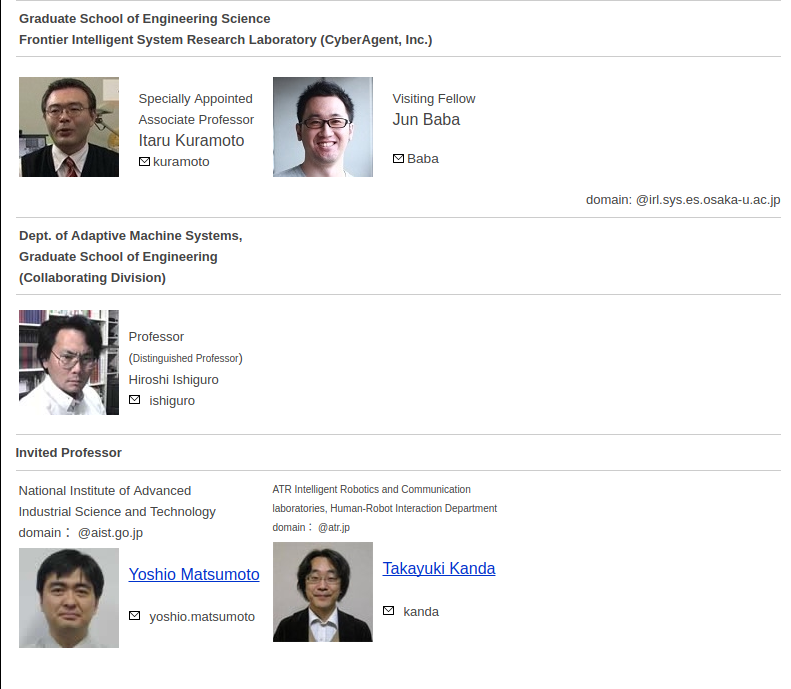
\includegraphics[width=1.0\textwidth]{pics/jap_intelligent_robotics_lab}
  \caption{Example of semi structured information}
\end{figure}

In order to understand the complexity of this extraction task take for example the
staff page for the intelligent robotics laboratory of Osaka University shown in figure 1.
Say we want to extract the name, position, email and picture of all members. It is easy to see
there is some sort of structure to the information we want to extract from this particular 
website, however, parts of the information are missing, repeated or disposed differently for
each particular member. If we want to go further it may be necessary to only extract information
from full members, a task that may pose a harder challenge. We may use grouping similarity 
combined with textual information in order to properly identify the desired entities.
In many cases the HTML element's relative position or CSS class name is sufficient to identify
particular occurrences of a same entity. If we do a good enough job at this first task we may 
extrapolate our model to extract information from similar web pages. 

However at this moment we are only interested in extracting researcher names and it is not
necessary to identify their status regarding full or partial membership.


Proposed solution

The name extraction problem is no different than a Named Entity Recognition problem, however 
approaches like Conditional Random Fields, Hidden Markov Models or Maximum Entropy Models that 
tipically achieve a high accuracy on free text perform very poorly in this particular case, 
because the data we are trying to extract is disposed in a tabular form and the words do not 
hold dependencies toward each other the same way they do in long pieces of text. Structural HTML
features and token probability distributions play a key role in the name extraction problem.

It is possible to solve the name extraction problem with a Bayesian statistical approach. 
But first lets define some notations: 

A simple Bayesian approach to solving the name extraction problem would be to calculate
the probability of a token being a name with the following expressions:

\[
P(is a name|token_n) = \frac{P(is a name) P(token_n|is a name)}{P(token_n)}
P(is not a name|token_n) = \frac{P(is not a name) P(token_n|is not a name)}{P(token_n)}
\]

Probabilities $ P(is a name), P(token_n|is a name) $ can be easily estimated, and, there
is no need to estimate $ {P(token_n)} $ since both scores will be divided by the same quantity.
However this model does not achieve a very good performance because it doesn't incorporate information
about surrounding tokens. Since name tokens are usually grouped together, it is expected that when
we know the previous tokens to be names the probability of the next token also being a name become higher. 
We can incorporate this knowledge in our expression and compute n-gram probabilities instead of 
unigrams: 

\[
P(w_1^{N}, ..., w_n^{N})
\]

Here we may use the probability chain rule to determine the window size with the assumption that
tokens outside that window have independent probability distributions. The sequence probability 
expression is given by:

\[
P(w_1^{N}, ..., w_n^{N}|w_1, ..., w_n) = \frac{P(w_1^{N}, ..., w_n^{N}) P(w_1, ..., w_n|w_1^{N}, ..., w_n^{N})}{P(w_1, ..., w_n)}
\]

We take here a simplifying assumption of conditional independence, otherwise it becomes hard
to obtain reliable probabilities.

$ P(w_1, ..., w_n|w_1^{N}, ..., w_n^{N}) = P(w_1|w_1^{N}) ... P(w_n|w_n^{N})$


So our expression becomes:

\[
P(w_1^{N}, ..., w_n^{N}|w_1, ..., w_n) = \frac{P(w_1^{N}, ..., w_n^{N}) P(w_1|w_1^{N})}...{P(w_n, w_n^N)}
\]

This is our base formula. Taking a window of size 4, we would need to estimate the probabilities:
P(NNNN) P(WWWW) ....

Most of the time, names are wholy contained inside a single html element, so it is useful to 
incorporate this evidence in our formula to delimit name boundaries. Instead of estimating P(NNNN)
we would need estimate P(N*NNN) P(NN*NN) etc.

Finally, we need to estimate the single token probabilities P(t|N) and P(t|W) and at this time
we may incorporate other sources of evidence as features in a Naive Bayes model. Some useful features
are token length and token incidence.

At this moment we still haven't incorporated any information about HTML structure in our model
besides the tag borders. Web page structure varies significantly among the different faculty
repositories, so it is hard to incorporate generalized features envolving HTML structure that
will perform well in most situations. 

Faculty repositories usually have names disposed in an ordery fashion. That means they share
similar attributes. If our crude model was able to find a relevant part of the names on the
first passing, we may improve its precision by estimating some structural attributes on this 
collection of names and using them to identify other names at a second passing.

Evaluation

The algorithm precision on the first passing is: .
The algorithm precision on the second passing is: .

Further research

The two passing strategy has potential to improve any data extraction task on semi structured
documents. It is out intent to explore it in different extraction scenarios.

\chapter{Schedule}

Schedule here.

% ==========================================
% End of text.                             |
% ==========================================

\ppgccbibliography{bibfile}
\nocite{*}

\end{document}
